\chapter{Symulacja komputerowa}
\section{Język i narzędzia programowania}
\hspace{4ex}Decyzja dotycząca wyboru platformy językowej była trudna. Pierwotnie mieliśmy skorzystać z takich języków wyższego rzędu jak JAVA, C\# ale w trakcie dyskusji o wymaganiach postawionych przed modelem aplikacji zmieniliśmy zdanie. Każdy język ma swoje mocne strony, ale w tym projekcie użyliśmy \emph{C$++11$} z następujących powodów:
\begin{enumerate}
  \item C++ jest językiem kompilowanym, co oznacza, że programy w nim działają bardzo szybko.
  \item C++ jest językiem wieloparadygmatowym, więc możemy programować proceduralnie, strukturalnie lub obiektowo.
  \item Duża różnorodność bibliotek oraz łatwość ich instalacji.
  \item Kompatybilność wsteczna z językiem C.
\end{enumerate}
\hspace{4ex}Ponadto korzystamy z zewnętrznych bibliotek(OpenGl: \emph{glut.h}) do obsługi renderowania symulacji, a także pakietu Qt do stworzenia UI aplikacji.
\section{Implementacja}
\subsection{Implementacja modelu}
\hspace{4ex}Do bezpośredniego renderowania animacji używamy biblioteki glut.h z pakietu OpenGL. Za sterowanie animacją odpowiada klasa QGLWidget dziedzicząca po klasie \emph{QOpenGLWidget}. Aby utworzyć prosty widget animacji, potrzebujemy nadpisać 3 metody: 
\begin{enumerate}
\item \emph{initializeGL()} - w której inicjalizujemy interfejs za pomocą metod biblioteki glut.h np.:
\item \emph{paintGL()} - w której umieszczamy metody rysujące pojedynczą klatkę animacji; metoda jest wywoływana przez QTimer co każde 10ms, 
\item \emph{resizeGL()} - która jest wywoływana przy zmianie rozmiaru okna aplikacji.
\end{enumerate}

Aby biblioteka \emph{glut.h} zaczęła działać musimy ją zainicjalizować w metodzie \emph{main.cpp}

\begin{lstlisting}
int main(int argc, char *argv[])
{
    //glut openGl initialization
    glutInit(&argc, argv);
    QApplication a(argc, argv);
    MainWindow w;
    w.show();

    return a.exec();
}
\end{lstlisting}

\hspace{4ex}Następnie budujemy główny obiekt zarządzający symulowaną sceną {SocialForce.h}, który inicjalizujemy z pliku XML. Szczegóły budowy w dalszej części. Najważniejszą metodą obiektu SocialForce jest \emph{makeAMove()}, która dostaje \emph{steptime} jak argument i dokonuje obliczenia sił, prędkości i położenia agentów po czasie \emph{stepTime}. Jeśli agent dotrze do celu (ostatniego WayPointa), jest on usuwany ze sceny symulacji.

\begin{lstlisting}
int numberOfAgent = myAgents.size();
for (int i = 0; i < numberOfAgent; i++){
	if (myAgents[i].getID() != -1){
        myAgents[i].makeAMove(myWalls, myAgents, stepTime);
        if (myAgents[i].isReachDestination())
            myAgents[i].setID(-1);
    }
}
\end{lstlisting}
\hspace{4ex}Dla każdego agenta obliczamy siły w celu obliczenia jego nowej lokalizacji. Do obliczeń użyliśmy wzorów, wypisanych wcześniej w części teoretycznej.

\begin{lstlisting}
forceWithWall = wallInteractForce(walls);
forceByThemselfe = internalForce();
forceWithOthers = agentInteractForce(agents);
acceleration =  forceByThemselfe + forceWithWall + forceWithOthers;

currentSpeed = currentSpeed*0.5 + acceleration * stepTime;
 
position = position + currentSpeed*stepTime;
\end{lstlisting}

\subsection{Interfejs użytkownika}
\hspace{4ex}Interfejs aplikacji zbudowany jest w oparciu o bibliotekę \emph{Qt} i środowisko \emph{Qt Creator}, które daje łatwość budowania intuicyjnych aplikacji okienkowych. Interfejs dostarcza użytkownikowi następujące możliwości:
\begin{enumerate}
\item wyświetlanie zewnętrznej siły działającej na agentów ze pomocą zmiany kolorów wyświetlania agentów (niebieski - najmniejsza siła, czerwony - największa siła),
\item wyświetlanie aktualnego wektora prędkości aktora,
\item wyświetlania waypoint'ów na scenie,
\item kalibracja współczynników sił działających na aktora: siły wewnętrznej, siły oddziaływania z innymi aktorami i siły oddziaływania z przeszkodami(ścianami),
\item zresetowanie współczynników do wartości początkowych,
\item zmiana czasu kroku symulacji jako \emph{stepTime}, dająca możliwość przyspieszania i zwalniania symulacji,
\item zatrzymania/wystartowanie symulacji
\item załadowania sceny symulacji z pliku .xml
\end{enumerate}

\begin{figure}[ht]
\centering
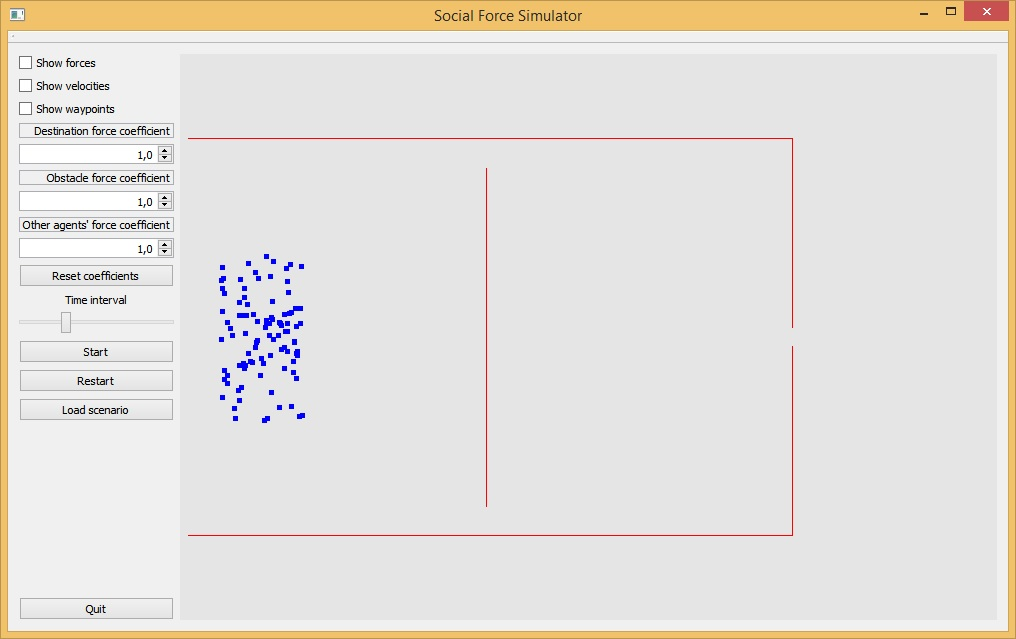
\includegraphics[scale=0.5]{ui}
\caption{Interfejs użytkownika}
\end{figure}

\subsection{Różnice implementacji w porównaniu z wersją książkową}
\hspace{4ex}Do obliczania siły interakcji pomiędzy agentem a agentami z otoczenia nie bierzemy pod uwagę wszystkich agentów ze sceny, tylko tych z najbliższego otoczenia.
Kolejną zmianą jest to, że do obliczenia sił interakcji uwzględniamy tylko najbliższą przeszkodę, a nie wszystkie znajdujące się na mapie. W wyniku symulacji zmieniliśmy też parametry siły interakcji z przeszkodami na $a=1.3$ i $b=0.8$. Symulacje na naszym modelu z książkowymi parametrami nie dawały satysfakcjonującego wyniku. Na agentów działało zbyt duże przyspieszenie, dlatego dodaliśmy do równania zmiany prędkości parametr $\alpha$
$$v_{new} = \alpha * v_{actual} + a * t $$
gdzie $\alpha = 0.5$

\subsection{Inicjalizowanie sceny}
\hspace{4ex}Jak już wcześniej wspomnieliśmy, inicjalizowanie sceny odbywa się z pliku w formacie XML.

Cały scenariusz zawiera się wewnątrz znacznika $<scenario> ... </scenario>$.

\subsubsection{Deklaracja waypoint'ów}
\hspace{4ex}Najpierw definiujemy waypoint'y, czyli punkty przez które muszą przejść agenci. Waypoint ma \emph{id}, współrzędne \emph{x} i \emph{y}, a także promień \emph{r}.

\begin{lstlisting}
  <waypoint id="1" x="-0.92" y="0" r="0.02" />
\end{lstlisting}

\subsubsection{Deklaracja agentów}
\hspace{4ex}Definowanie agenta jest trochę bardziej skomplikowane. Każdy agent posiada współrzędne \emph{x} i \emph{y} oraz liczbę generowanych agentów \emph{n} i parametry \emph{dx} i \emph{dy}. \emph{n} agentów jest generowanych ze współrzędnymi początkowymi $(x \pm dx, y \pm dy)$. Dodatkowo dla tych agentów dodaje się waypointy za pomocą znacznika $<addwaypoint ... />$ z \emph{id} waypointa, które musi się zgadzać, z którymś z waypoint'ów zadeklarowanych wcześniej. Kolejność dodawania waypoint'ów jest istotna; w takiej kolejności będą zmierzali do nich agenci. Całość definicji agenta zamykamy w znaczniku $<agent> ... </agent>$. Przykład:

\begin{lstlisting}
<agent x="-0.7" y="0" n="100" dx="0.2" dy="0.4">
    <addwaypoint id="2" />
</agent>
\end{lstlisting}

\subsubsection{Deklaracja przeszkód(ścian)}
\hspace{4ex}Ostatnim elementem jest zadeklarowanie ścian $<obstacle ... />$.
Zawiera on współrzędne \emph{x1, y1} początku ściany oraz współrzędne \emph{x2,y2} końca ściany.

\begin{lstlisting}
 <obstacle x1="-0.9" y1="-0.9" x2="-0.9" y2="-0.03" />
\end{lstlisting}




\subsubsection{Przykładowa deklaracja scenariusza}

\begin{lstlisting}
<scenario>
  <waypoint id="1" x="-0.92" y="0" r="0.02" />
  <waypoint id="2" x="0.92" y="0" r="0.02" />
  
  <agent x="-0.7" y="0" n="100" dx="0.2" dy="0.4">
    <addwaypoint id="2" />
  </agent>
  <agent x="0.7" y="0" n="100" dx="0.2" dy="0.4">
    <addwaypoint id="1" />
  </agent>
  
  <obstacle x1="-0.9" y1="-0.9" x2="-0.9" y2="-0.03" />
  <obstacle x1="-0.9" y1="0.03" x2="-0.9" y2="0.9" />
  <obstacle x1="-0.9" y1="-0.9" x2="0.9" y2="-0.9" />
  <obstacle x1="-0.9" y1="0.9" x2="0.9" y2="0.9" />
  <obstacle x1="0.9" y1="-0.9" x2="0.9" y2="-0.03" />
  <obstacle x1="0.9" y1="0.03" x2="0.9" y2="0.9" />	
</scenario>
\end{lstlisting}


\newpage
\section{Diagramy klas UML}
\hspace{4ex}
\begin{figure}[ht]
\centering
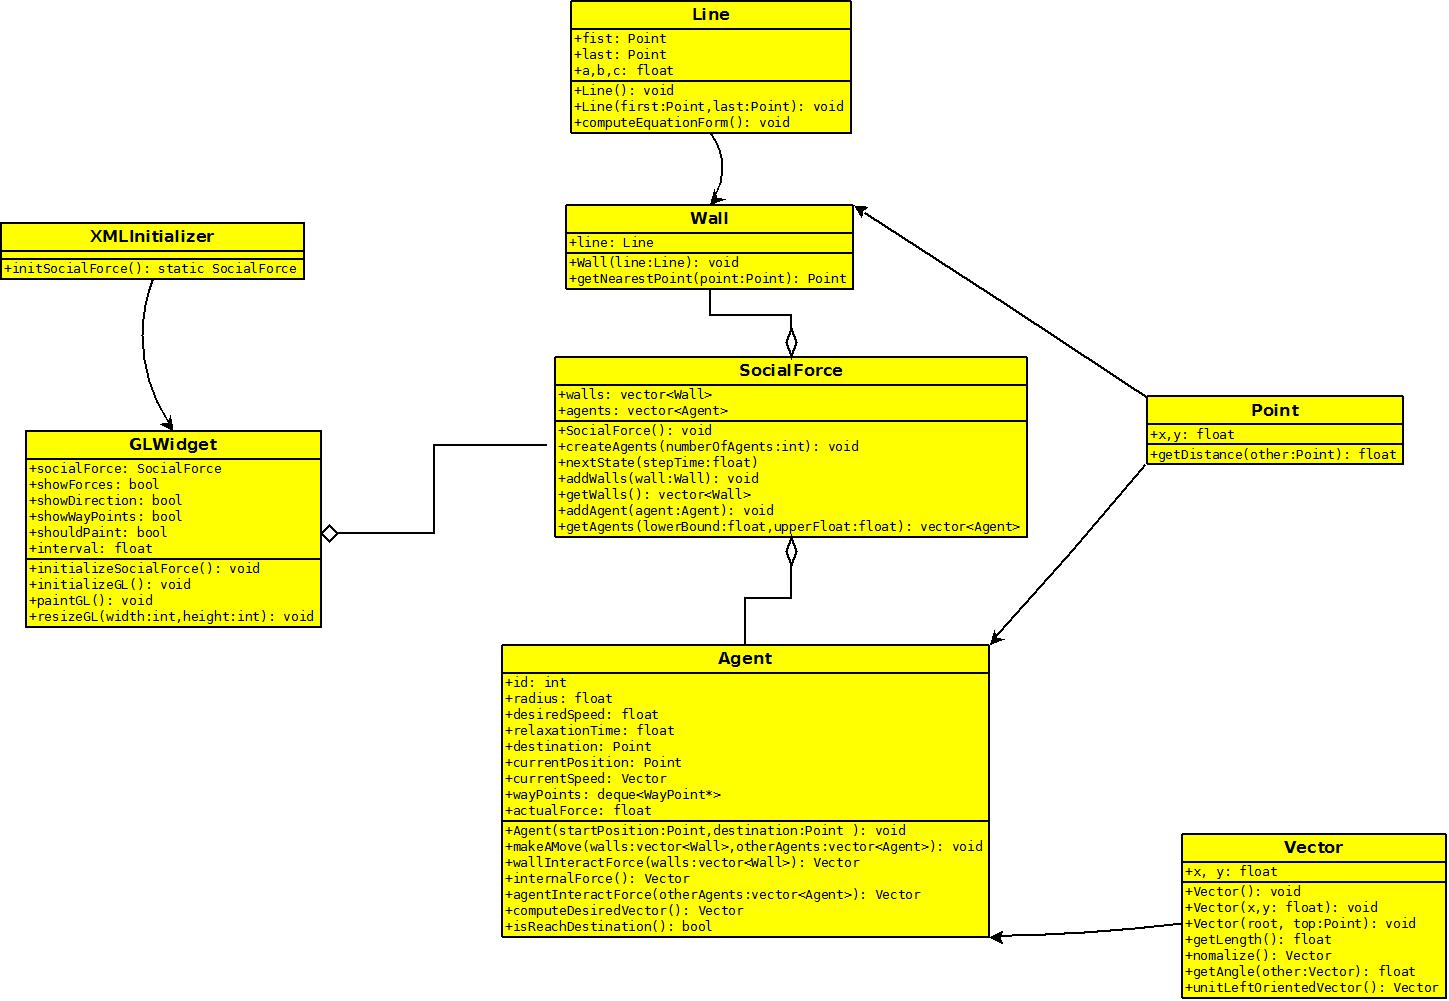
\includegraphics[scale=0.4]{ClassDiagram}
\caption{Diagram klas}
\end{figure}